\documentclass[tikz,border=1.5pt]{standalone}
\newif\ifko \kofalse

% style.tex — 구성도 공용 (standalone, xelatex). \kotrue / \kofalse 를 먼저 정함.
\usepackage{mathptmx}
\usepackage[no-math]{fontspec}
\setmainfont{TeX Gyre Heros}
\ifko
  \newfontfamily\krfont{Noto Sans CJK KR}[Scale=0.9]
  \usepackage[Latin,Korean]{ucharclasses}
  \setTransitionsForKorean{\begingroup\krfont}{\endgroup}
\fi
\usepackage{xcolor}
\definecolor{cFRiii}{HTML}{0072B2}
\definecolor{cFRv}{HTML}{D55E00}
\definecolor{cEmph}{HTML}{009E73}
\usepackage{tikz}
\usetikzlibrary{positioning,fit,backgrounds,arrows.meta,calc,shapes.geometric,shapes.misc,decorations.pathreplacing}
\newcommand{\T}[2]{\ifko #1\else #2\fi}
\tikzset{
  >={Stealth[length=2.2mm,width=1.6mm]},
  every node/.style={font=\fontsize{7.2}{8.6}\selectfont},
  box/.style={draw=black, line width=0.5pt, rounded corners=1.2pt, fill=white, align=center, inner sep=2.6pt, minimum height=8.5mm, text width=#1},
  box/.default=24mm,
  gbox/.style={box=#1, fill=black!6},
  gbox/.default=24mm,
  ebox/.style={box=#1, draw=cEmph, line width=1.0pt, fill=cEmph!7},
  ebox/.default=24mm,
  grp/.style={draw=black!55, dashed, line width=0.45pt, rounded corners=2pt, inner sep=3.2mm},
  grplabel/.style={anchor=north west, font=\fontsize{7.6}{9}\selectfont\bfseries, inner sep=1.2pt, fill=white},
  ar/.style={->, line width=0.6pt},
  ear/.style={->, line width=1.1pt, draw=cEmph},
  dar/.style={->, line width=0.55pt, dashed},
  small/.style={font=\fontsize{6.3}{7.4}\selectfont},
  lab/.style={font=\fontsize{6.3}{7.4}\selectfont, fill=white, inner sep=1pt},
}
\newcommand{\D}{\fontsize{6.3}{7.5}\selectfont\color{black!78}}
\newcommand{\code}[1]{\texttt{#1}}

\begin{document}
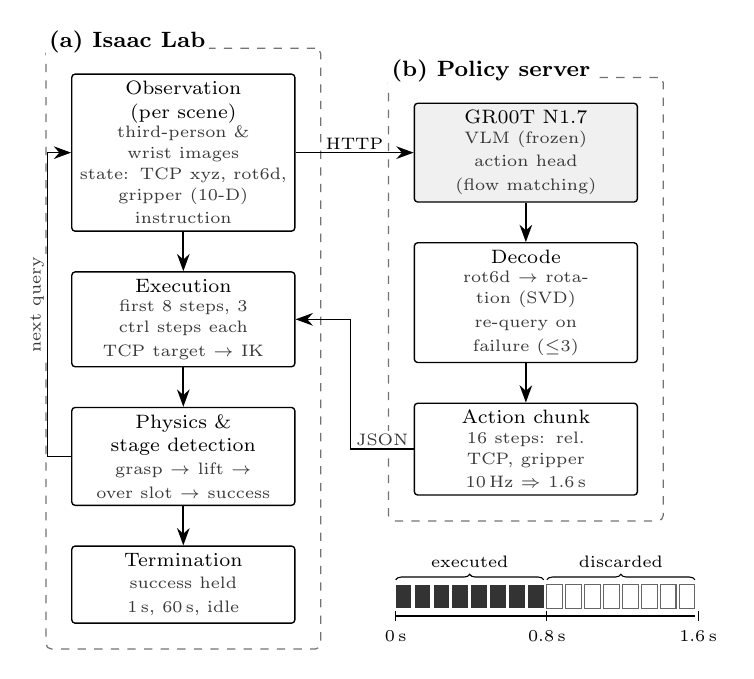
\begin{tikzpicture}[node distance=5mm]
\def\W{26.5mm}
% ---------------- 워크스테이션: Isaac Lab
\node[box=\W, anchor=north west] (o) at (0,0) {\T{관측 (장면마다)}{Observation (per scene)}\\[-0.5pt]{\D\T{3인칭 $\cdot$ 손목 화면}{third-person \& wrist images}\\\T{상태: 손끝 xyz, rot6d,\\그리퍼 (10)}{state: TCP xyz, rot6d,\\gripper (10-D)}\\\T{지시문}{instruction}}};
\node[box=\W, below=of o] (x) {\T{실행}{Execution}\\[-0.5pt]{\D\T{앞 8칸, 칸마다 3 스텝}{first 8 steps, 3 ctrl steps each}\\\T{손끝 목표 $\rightarrow$ 역기구학}{TCP target $\rightarrow$ IK}}};
\node[box=\W, below=of x] (p) {\T{물리 $\cdot$ 단계 판정}{Physics \& stage detection}\\[-0.5pt]{\D\T{쥠 $\rightarrow$ 들어 올림 $\rightarrow$ 슬롯 위 $\rightarrow$ 성공}{grasp $\rightarrow$ lift $\rightarrow$ over slot $\rightarrow$ success}}};
\node[box=\W, below=of p] (e) {\T{끝나는 조건}{Termination}\\[-0.5pt]{\D\T{성공 1 s 유지 $\cdot$ 60 s $\cdot$ 멈춤}{success held 1\,s, 60\,s, idle}}};
\draw[ar] (o) -- (x); \draw[ar] (x) -- (p); \draw[ar] (p) -- (e);
\draw[ar] (p.west) -- ++(-3mm,0) |- node[lab, pos=0.25, rotate=90, above]{\D\T{다음 물음}{next query}} (o.west);
% ---------------- 학습 서버: 정책
\node[gbox=\W, right=15mm of o] (s1) {GR00T N1.7\\[-0.5pt]{\D\T{VLM (고정)}{VLM (frozen)}\\\T{행동 헤드 (flow matching)}{action head (flow matching)}}};
\node[box=\W, below=of s1] (s2) {\T{풀기 (decode)}{Decode}\\[-0.5pt]{\D\T{rot6d $\rightarrow$ 회전 (SVD)}{rot6d $\rightarrow$ rotation (SVD)}\\\T{실패면 다시 물음 (3번)}{re-query on failure ($\le$3)}}};
\node[box=\W, below=of s2] (s3) {\T{행동 묶음}{Action chunk}\\[-0.5pt]{\D\T{16칸: 손끝 상대값, 그리퍼}{16 steps: rel.\ TCP, gripper}\\10\,Hz $\Rightarrow$ 1.6\,s}};
\draw[ar] (s1) -- (s2); \draw[ar] (s2) -- (s3);
\draw[ar] (o.east) -- node[lab, above]{HTTP} (s1.west);
\draw[ar] (s3.west) -- node[lab, above]{\D JSON} ++(-8mm,0) |- (x.east);
\begin{scope}[on background layer]
\node[grp, fit=(o)(e)] (GW) {};
\node[grp, fit=(s1)(s3)] (GS) {};
\end{scope}
\node[grplabel] at ($(GW.north west)+(0,2.6mm)$) {(a) Isaac Lab};
\node[grplabel] at ($(GS.north west)+(0,2.6mm)$) {(b) \T{정책 서버}{Policy server}};
% ---------------- 묶음 시간 줄
\begin{scope}[shift={($(GS.south west)+(1mm,-11mm)$)}]
\def\cw{2.4mm}
\foreach \i in {0,...,15} {
  \ifnum\i<8 \fill[black!80] (\i*\cw,0) rectangle ++(\cw-0.4mm,3mm);
  \else \draw[black!60, line width=0.4pt] (\i*\cw,0) rectangle ++(\cw-0.4mm,3mm); \fi }
\draw[line width=0.4pt] (0,-1mm) -- (16*\cw-0.4mm,-1mm);
\foreach \i/\t in {0/0, 8/0.8, 16/1.6} \draw (\i*\cw,-0.4mm) -- (\i*\cw,-1.6mm) node[below, small] {\t\,s};
\draw[decorate, decoration={brace, amplitude=2pt}] (0,3.6mm) -- node[above, small, yshift=1pt]{\T{실행}{executed}} (8*\cw-0.4mm,3.6mm);
\draw[decorate, decoration={brace, amplitude=2pt}] (8*\cw,3.6mm) -- node[above, small, yshift=1pt]{\T{버림}{discarded}} (16*\cw-0.4mm,3.6mm);
\end{scope}
\end{tikzpicture}
\end{document}
